\documentclass[]{article}

\usepackage{graphicx}
\usepackage[english]{babel}
\usepackage{wrapfig}
\usepackage[top=1in, bottom=1.25in, left=1.25in, right=1.25in]{geometry}
\usepackage{setspace}
\usepackage[utf8]{inputenc}
\usepackage{dirtytalk}
\usepackage[backend=bibtex,citestyle=authoryear,url=false,doi=true]{biblatex}
\addbibresource{ZoteroBib.bib}
\usepackage[section]{placeins}

%opening
\title{Agency, Consent, Schizophrenia}
\author{Alec J Hoyland}
\doublespacing

\begin{document}

\maketitle

\begin{abstract}

	In partial fulfillment of the History of Ideas minor at Brandeis University, I present this manuscript discussing the genealogy of schizophrenia as a scientific phenomenon and discuss the intersection of genealogy, science, and social justice. What philosophical and sociological conclusions can we gather from current neuroscientific research? This work is broken into three parts. First we consider the scientific and philosophical implications of anomalous self-experience in schizophrenia. Second, we consider an examination of agency in schizophrenic individuals. Finally, we consider the implications of the first and second sections on issues of social justice concerning sexual consent. Throughout this small work, I have included drawings and paintings by schizophrenic painters. 

\end{abstract}

\begin{figure}
	\centering
	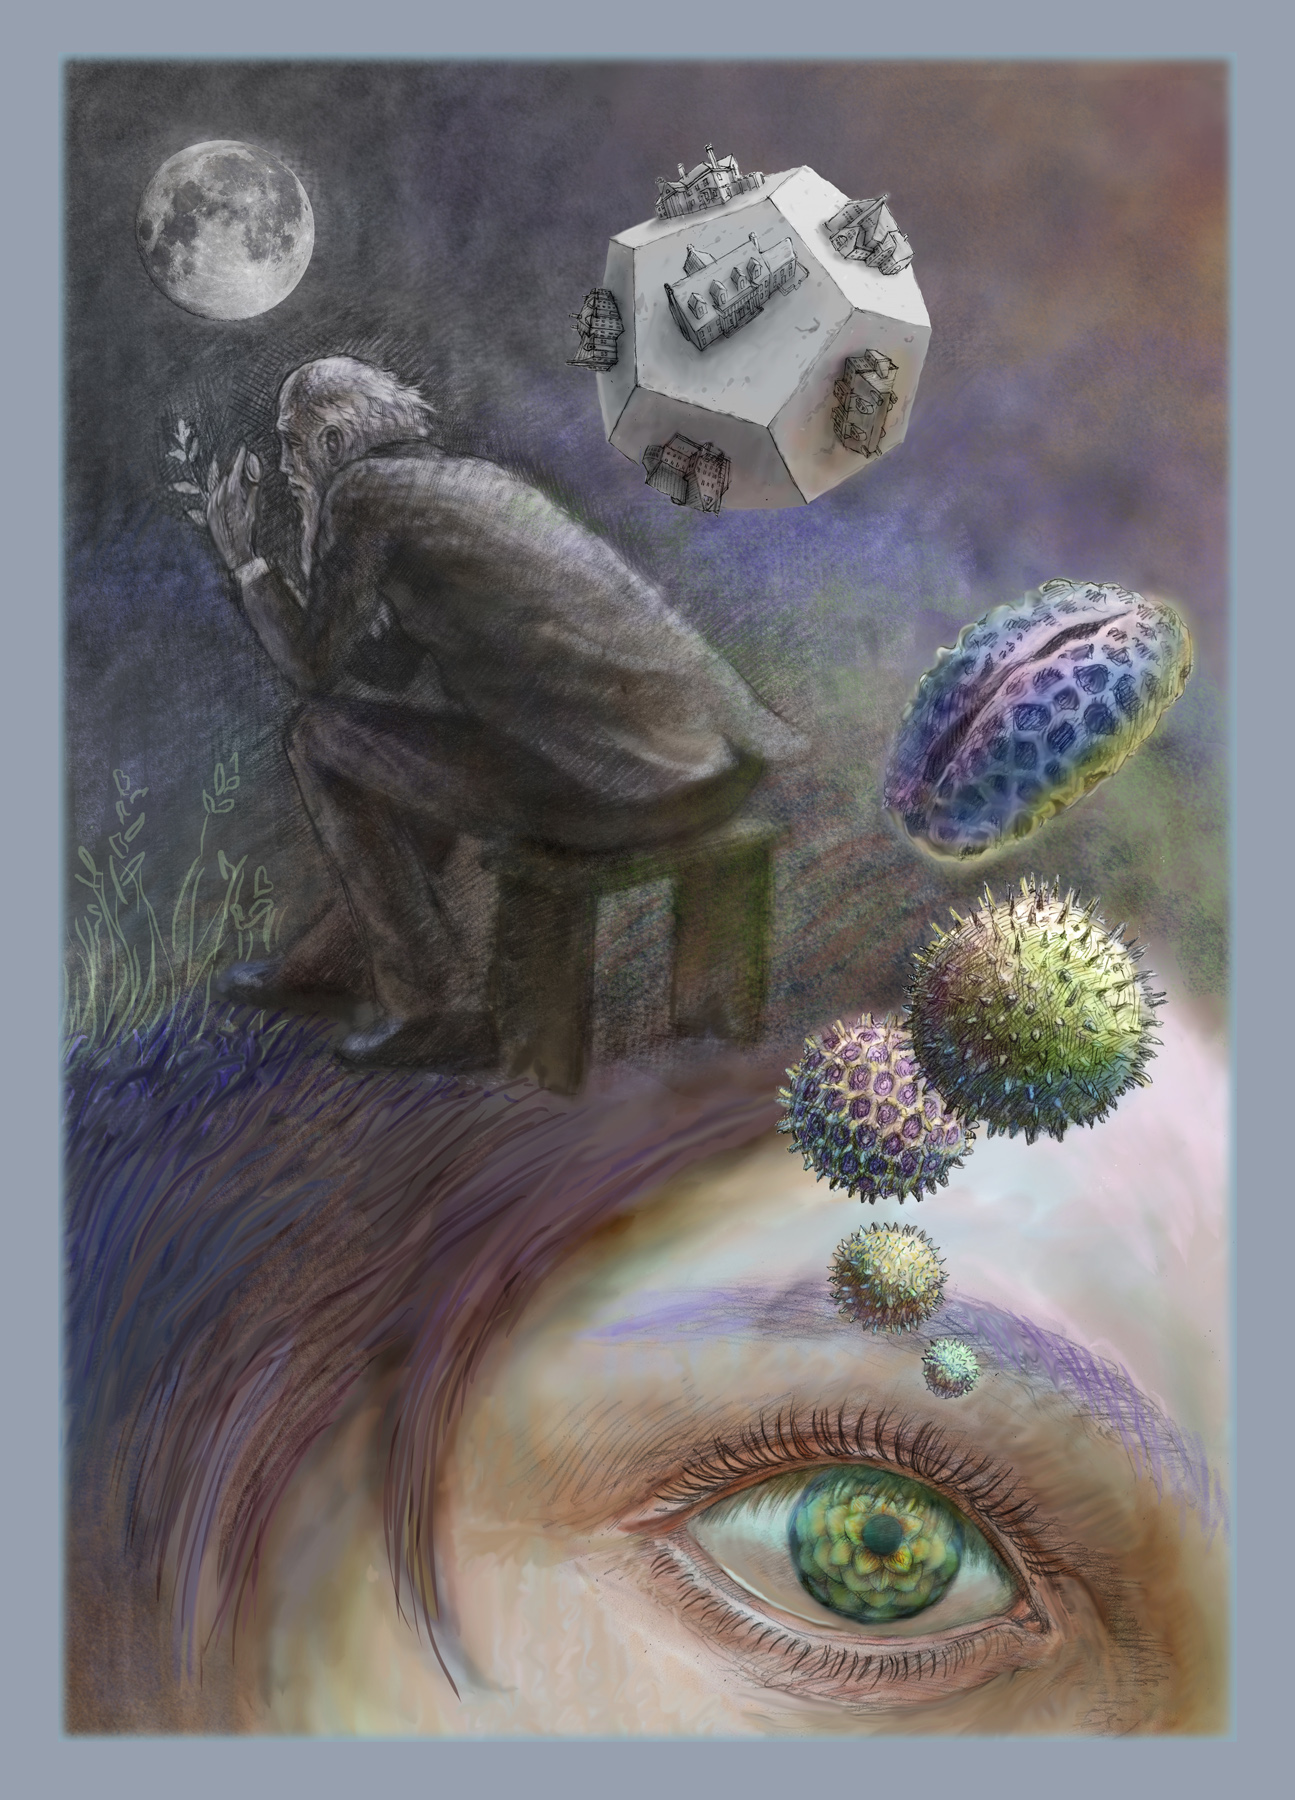
\includegraphics[width=0.8\textwidth]{graphics/BenMarder1}
	\caption{Pencil by Ben Marder}
\end{figure}


\section{Anomalous Self Experience in Schizophrenia}

	\subsection{Introduction}
		
		We find ourselves at a unique and incontrovertibly fascinating point in human history, in which the methods and will to discover the governing physical principles of the brain and nervous system are finally within our grasp. The twentieth century provided great leaps in microscopy, electrophysiology, and computation spring-boarding on the revolutionary insights of Cajal and Golgi. Models of neuronal activation and memory advanced the understanding of neuronal communication and assembly; though it was not until the later quartile that work in human neuropsychiatry meaningfully began in earnest. 
		
		For so long, the schizophrenic has been exploited as a secret weapon of continental philosophy. Foucault lauded the schizophrenic and criticized the medical orthodoxy of the \say{great confinement.} Deleuze deified the schizophrenic in \textit{Capitalism \& Schizophrenia}, in which they became a model of freedom from psychosexual power dynamics that subjugate the Western capitalist state.
		
		I attempt to rectify the intellectual achievements of the twentieth-century luminaries with modern neuroscientific theories regarding the etiology and pathology of schizophrenia.
		
		In this first section, I wish to elucidate some of the more salient points discussing schizophrenia as a mental illness as currently understood by psychiatry and neuroscience. 
	
	
	\subsection{Schizophrenia as a Medico-Scientific Phenomenon}
		
		Schizophrenia is a severe, chronic neuropsychiatric disorder affecting 1\% of the world population characterized by psychosis, neurocognitive deficits, and negative symptoms ranging from anhedonia, flat affect, and asocial behavior. Schizophrenia typical onsets during young adulthood, following a prodromal period of subacute cognitive deficits and negative symptoms, characterized by a psychotic break. Common symptoms include false beliefs, unclear thinking, hallucinations, reduced social engagement, emotional expression, and lack of motivation (\cite{TandonSchizophreniajustfacts2009,HinchliffSynthesisphylogenytaxonomy2015}).
		
		The precise causes of schizophrenia are unknown. Potential causes include variegated environmental and genetic factors. City living, viral infections, cannabis use, and diathesis have been noted (\cite{HinchliffSynthesisphylogenytaxonomy2015,ChadwickCannabisUseAdolescent2013}).
		
		In modern clinics, diagnosis is based upon observed behavior, testimony from the patient and those close to them, and cultural factors. Contrary to popular discourse, schizophrenia does not imply a \say{split personality} or other dissociative disorder.
		
		\begin{figure}
			\centering
			
\includegraphics[width=0.5\textwidth]{graphics/DortheRandiSchmidt3}
			\caption{Pencil by Dorthe Randi Schmidt}
		\end{figure}
		
		Treatment generally consists of psychotherapy, antipsychotic medication, and hospitalization. Social problems, such as long-term unemployment, poverty, homelessness, and drug use are common. While about 20\% of schizophrenics recover completely (full remission), the life expectancy for schizophrenics is cut by ten to twenty-five years. This is due to increased risk of physical health problems and suicide rate 300 times larger than the national average (\cite{HinchliffSynthesisphylogenytaxonomy2015,FosterHomelessnessSchizophrenia2012,OsSchizophrenia2009}).
		
		There are no reliable biological markers of schizophrenia, thought neuroimaging and neuroanatomical studies have correlated reductions in synaptic density in the prefrontal cortex and temporal lobes with onset of the prodromal period (\cite{RimolCorticalThicknessSubcortical2010,GlantzLADecreaseddendriticspine2000,HillMolecularmechanismscontributing2006,BuckleyNeuroimagingschizophreniastructural2005,FaludiSynapticchangesbrain2011,BoksaAbnormalsynapticpruning2012,PalaniyappanStructuralcorrelatesformal2015}).
		
		\begin{figure}
			\centering
			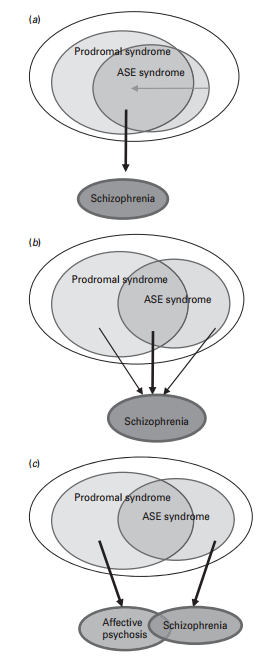
\includegraphics[width=0.5\textwidth]{graphics/ModelingSchizophreniformPathogenesis}
			\caption{Modeling schizophreniform pathogenesis (Parnas 2009).}
		\end{figure}
		
		Anomalous self-experiences (ASE, self-disorders) have also been identified as unique to schizophrenia among psychotic disorders (\cite{ParnasPhenomenologyanomalousselfexperience2003,ParnasDisorderedSelfSchizophrenia2014}). The Examination of Anomalous Self-Experience (EASE) has been identified as a credible method for assessing psychopathological self-experiences (\cite{ParnasEASEExaminationAnomalous2005,MollerExaminationAnomalousSelfExperience2011}). Direct correlation between severity of prodromal psychosis as rated symptomatically and anomalous self-experience indicates that insidious onset schizophrenia presents with greater frequency (\cite{BrentSelfDisturbancesPossiblePremorbid2014,KorenDisturbancesbasicself2013}).
		
		The medial prefrontal cortex is thought to be involved in the process of self-reference. Schizophrenics show increased activation in the right dorsomedial prefrontal cortex and left ventromedial prefrontal cortex when describing themselves in positive terms and abnormally high activation in the right dorsomedial prefrontal cortex when describing themselves negatively (\cite{PfeiferKnowYouAre2007,ModinosSelfreflectionpsychosispronebrain2011}). In addition, schizophrenics show reduced default-mode network connectivity in the dorsomedial prefrontal cortex, but not in bipolar disorder (\cite{OngurDefaultmodenetwork2010}).
		
	\subsection{Anomalous Self-Experience}
	
		From a genealogical perspective, the development of the EASE is quite interesting. The original scientific paper was published in 2005 in the clinical journal \textit{Psychopathology}. It was predominately a northern European endeavor, with researchers at the Universities of Aachen and Copenhagen. In fact, the development of the EASE scale heralded the first major work published by the novel Center for Subjectivity Research at the University of Copenhagen. Led by the charming phenomenologist Dan Zahavi, the Center studies scientific and medical problems of subjectivity and thus the sane and the insane. This endeavor of scientific inquiry with philosopher banner-heads hearkens back to an Old World approach to scholarship.
	
		Trained as a Husserlian phenomenologist, Zahavi has argued for the necessity of phenomenological considerations in twenty-first century cognitive science (Zahavi x3). Just as classical psychology has bowed to neuroscience, psychophysics, and statistical physics approaches, so too must the hierarchical norms of traditional psychology accept the scholastic leadership of phenomenal metacogitators. The Center for Subjectivity Research approaches the comprehension and treatment of psychiatric disorders such as schizophrenia, autism, and anxiety as well as renovations of pre-modern introspectives (Hegel, Husserl, Heidegger, etc.).
		
		\begin{figure}
			\centering
			
\includegraphics[width=0.5\textwidth]{graphics/DortheRandiSchmidt2}
			\caption{Pencil by Dorthe Randi Schmidt}
		\end{figure}
		
		
		I do not wish to imply that this paradigmatic shift in psychiatric research into disorders of the self is entirely the endeavor of Zahavi. The advisory board at the Center for Subjectivity Research consists of Ingolf U. Dalferth, G\"{u}nter Figal, Shaun Gallagher, Axel Honneth, Alva No\"{e}, Philippe Rochat, Louis Sass, Galen Strawson, and Evan Thompson.
		
		From the perspective of a historian, philosopher, genealogist, an understanding of psychiatry might go as follows. There was a period of great not-knowing during the pre-Renaissance era in which madness was romanticized, feared, or both (\cite{DiamondAngerMadnessDaimonic1996}). Dante Alighieri writes in \textit{Purgatorio} that,
		
		\begin{quote}
			Madness it is to hope that human minds can ever understand the Infinite that comprehends Three Persons in One Being.
		\end{quote}
		
		Here of course, he makes reference to Christian doctrine and the triangular fetishism which has pervaded all human societies. More so to our interests, he depicts an understanding of madness which describes attempting to understand the whole of an infinite thing at once. We may take this to mean the madness of Georg Cantor or perhaps Ludwig Boltzmann, or perhaps that things can only be comprehended in hyperplane. By this I mean that any understanding should bastardize or otherwise irreconcilably reduce the object of our examinations. This concept comes to us through Plato, Dante, and even Nietzsche. When we attempt to perceive and thence understand, we will forever be grasping at phantoms.
		
		Perhaps a more recent interpretation may be of help. As Douglas Adams puts it,
		
		\begin{quote}
			Let's think the unthinkable, let's do the undoable. Let us prepare to grapple with the ineffable itself, and see if we may not eff it after all.
		\end{quote}
	
		Subjectivity is one of these terribly difficult things to grasp. The EASE represents a remarkable development in the clinical interpretation of schizophrenia. This revolution would not come for some time however. Foucault describes the Great Confinement in \textit{Madness and Civilization}, in which the luminaries of the age of reason opted to do the 'humane thing' and separate the insane from the sane. In contrast to reason and Western-Christian decency, prostitutes, vagrants, blasphemers, and the mad chose their unwholesome path. Those afflicted with unreason would therefore be confined until such time that they could be redeemed and released back into the general population.
		
		As with all reactionary extra-judicial political maneuvering, this served the twin purposes of social and economic expediency and would be reexamined later with a combination of guilt and righteousness. The confined could work without pay for the wardens and a terrible suffering would be swept from the streets of good and lawful society. The first bricks in the foundation of psychiatry were laid here. Madness became an object of empirical examination. The patient-inmates were research subjects. It is difficult to tell whether these methods were effective.
		
		\begin{figure}
			\centering
			
\includegraphics[width=0.5\textwidth]{graphics/DortheRandiSchmidt1}
			\caption{Pencil by Dorthe Randi Schmidt}
		\end{figure}
		
		
		Certainly Philippe Pinel humanized and codified the treatment of the mentally ill. His banishment of bleeding, purging, blistering, and chaining to the sordid and unscientific annals of medievalist medicine began a glorious career in the treatment of the insane. One of the last great nosologists of the eighteenth century (alongside Emil Kraepelin), Pinel attempted to treat madness as a moral disease. His firm, moral-figure treatments were certainly far more successful than the previous attempted at what amounted to civilized trepanation. Pinel maintains the honor of founding the modern principles of psychiatry. By this I do not mean the principles of cognitive science or psychology, but the true etymological definition of \say{healing the mind.}
		
		\FloatBarrier
		
		Hegel reports upon Pinel, saying,
		
		\begin{quote}
			The right psychical treatment therefore keeps in view the truth that insanity is not an abstract loss of reason (neither in the point of intelligence nor of will and its responsibility), but only derangement, only a contradiction in a still subsisting reason; just as physical disease is not an abstract, i.e. mere and total, loss of health (if it were that, it would be death), but a contradiction in it. This humane treatment, no less benevolent than reasonable (the services of Pinel towards which deserve the highest acknowledgement), presupposes the patient's rationality, and in that assumption has the sound basis for dealing with him on this side just as in the case of bodily disease the physician bases his treatment on the vitality which as such still contains health.
		\end{quote}
		
		Foucault deserves all the criticisms he gets for his factual errors, but that is not the point. Instead, he attempts to evaluate some of the more salient problems in modern (mid-twentieth century) psychiatry by tracing the ideas through history. In many ways Foucault is the \textit{wunderkind} for the anti-psychiatry movement of the 1960s. 
		
		Prominent psychiatrists such as Thomas Szasz (in \textit{The Myth of Mental Illness}) criticized the medical establishment for the \say{pharmocratic} pathologization of problems in living. One of the more nuanced libertarian intellectuals of the twentieth century, Szasz spoke out against the pathologization, persecution, and restriction of personal freedoms afforded to the mentally ill. While many of his ideas, like Foucault's, were founded on faulty ideas (cf. Schaler 2005 \say{The Myth of Mental Illness}), the principle remains: something is rotten in the state of psychiatry.
		
		It is customary at this time to mention \textit{On Being Sane in Insane Places} by David Rosenhan as published in the esteemed journal \textit{Science}, but the paper is so profoundly facile and unscientific that I cannot bear myself to even refute it. As the apocryphal quote attributed to Wolfgang Pauli, \say{That is not only not right; it is not even wrong!}
		
		An examination of the known science and amoral capitalism of pharmaceutical companies during the mid-twentieth century indicates that Foucault and contemporaries are, as the saying goes, \say{not wrong.}
		
		\begin{figure}
			\centering
			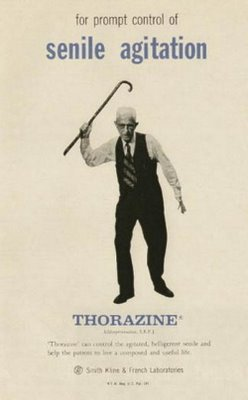
\includegraphics[width=0.5\textwidth]{graphics/ThorazineAdvertisement1}
			\caption{Typical anti-psychotic drug advertisement (Smith Kline \& French Laboratories, c. 1960)}
		\end{figure}
		
		It is for this reason, that I consider modern psychiatry to have begun (in the United States) with the \textit{Diagnostic and Statistical Manual of Mental Disorders IV}. The original fourth edition of the manual was published by the American Psychiatric Association in 1994. A text-revision (\textit{DSM IV-TR}) was published in 2000 to keep the DSM at least nominally in line with the \textit{International Classification of Diseases 10}, published by the World Health Organization, and used by the rest of the world.
		
		By the turn-of-the-century, novel scientific methods viz. magnetic resonance imaging/nuclear magnetic resonance (MRI/NMR), cloning, induced pluripotent stem cells (iPSCs) had turned the clinic from a place of convalescence and confinement to a functioning medical apparatus with revolutionary medical techniques bolstered by scientific principles. These advances came from basic biological research over the past century. New medications are significantly more successful than the \say{typical} anti-psychotics of the last mid-century. While the tools, tricks, and technologies of psychiatry had improved, the basic foundational principles of treatment had not. It cannot be understated how important scientific advancements were to the ability of mental health professionals to perform their tasks effectively. In the 1960s, it was appropriate to refer to schizophrenia in flowery post-modernist language (cf. \textit{Capitalism \& Schizophrenia} by Gilles Deleuze and F\'elix Guattari). This was possible because the psychiatric establishment was incapable of responding in a meaningful manner. Yet, as the philosophy of mind gave way to neurophilosophy, the poetic claims of anti-psychiatry withered as well.
		
		Thus, it is all the more remarkable that philosophers have remained such an important bulwark of theoretical neuroscience. The success of the EASE in helping patients has, in many ways, provided a syncretic clarion call for tackling the most difficult questions of selfhood, subjectivity, and sanity within the framework of empirical reality.
		
		
	\subsection{Synaptic Elimination}
		
		In healthy individuals, the human genome produces a consistent molecular architecture in the prefrontal cortex despite variegated genetic differences between individuals and populations. Evidence suggests disruptions in enzymes and metabolites mediate overzealous synaptic pruning in schizophrenic individuals.
		
		Rho GTPases are G-protein-activating kinases which regulate the actin cytoskeleton and control the structural remodeling and formation of synapses. Rho GTPase regulatory proteins direct synapse development and plasticity by controlling the spatio-temporal regulation and signaling specificity of Rho GTPases (\cite{ToliasControlsynapsedevelopment2011}). Tissue sections of dorsolateral prefrontal cortex (Brodmann area 9) from schizophrenia patients processed with fluorescent \textit{in-situ} hybridization (FISH) correlated messenger RNA (mRNA) expression of Rho GTPases to synaptic spine density (\cite{BoksaAbnormalsynapticpruning2012,HillMolecularmechanismscontributing2006}). Glutamine/glutamate (Glx) and N-acetylaspartate (NAA) levels in the dorsolateral prefrontal cortex were found to be elevated in young adulthood among attenuated and first-episode psychotics (schizophrenia spectrum). Glutamate serves as an excitatory neurotransmitter and NAA is a metabolite thought to be an indicator of neuronal metabolism (\cite{BoksaAbnormalsynapticpruning2012}). An $H^1-MRS$ study concluded that attenuated and first-episode patients showed an increase in Glx and NAA (\cite{LiemburgPrefrontalNAAGlx2016}).
		
		\begin{figure}
			\centering
			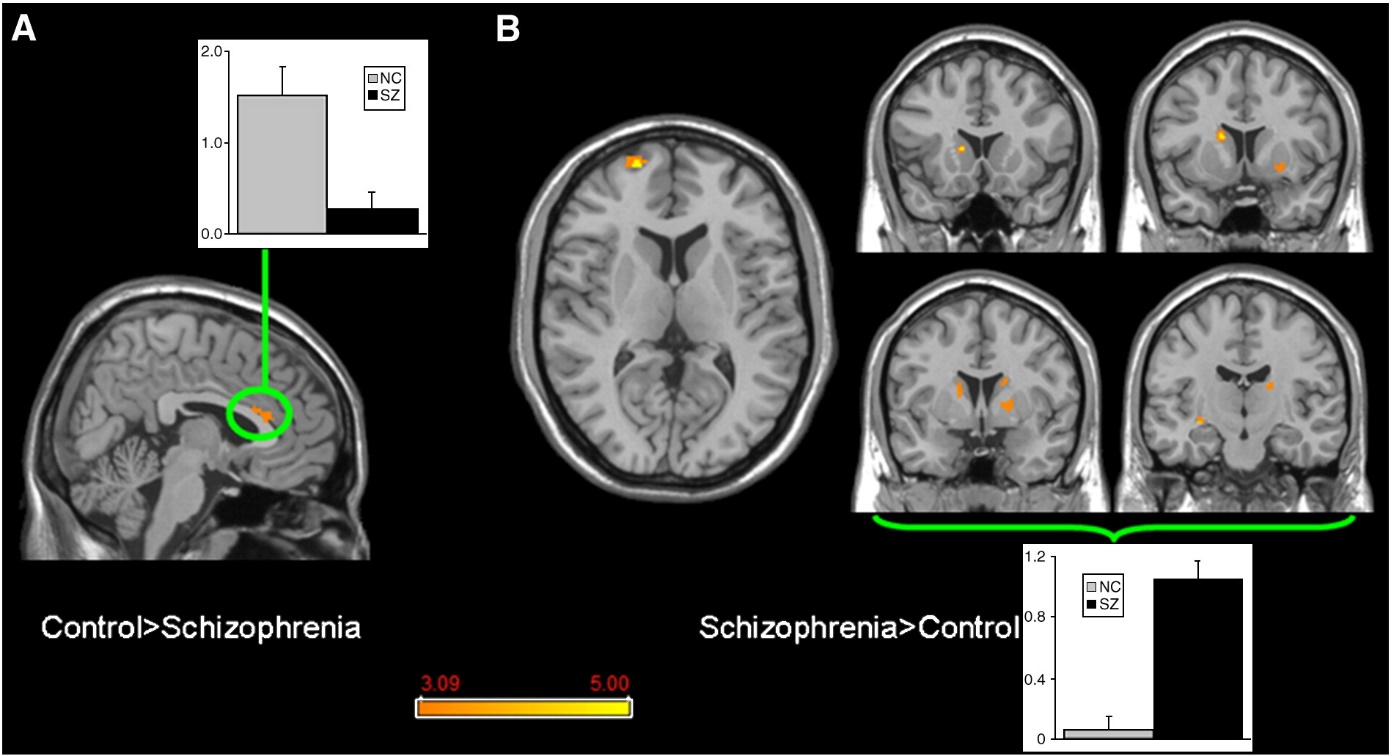
\includegraphics[width=0.8\textwidth]{graphics/AbnormalitiesNeuralActivity}
			\caption{Abnormalities in neural activity in schizophrenia. The schizophrenic brain exhibits abnormal activation in the medial prefrontal cortex (\cite{OngurDefaultmodenetwork2010}).}
		\end{figure}	
		
		In a study of 65,000 subjects, the C4 alleles of the major histocompatibility complex on chromosome 6 were highly correlated with schizophrenia. The alleles associated with schizophrenia risk were in direct proportion to its effect on C4A expression. C4 is expressed by neurons and localized to synapses. In mouse models, C4 promoted synapse elimination in temporally localized neurodevelopment of a neuronal circuit. The late phase of cortical maturation in humans corresponds to the same period of prodromal and first-episode schizophrenia. Complement receptors for the C4 protein are primarily expressed by microglia (phagocytic immunocytes in the CNS) (\cite{SekarSchizophreniariskcomplex2016}).
		
		\begin{figure}
			\centering
			\includegraphics*[width=0.8\textwidth]{graphics/MajorHistocompatibilityComplex}
			\caption{MHC signal is strongly correlated with schizophreniform pathology (\cite{SekarSchizophreniariskcomplex2016}).}
		\end{figure}
		
	\subsection{A Humble Hypothesis}
		
		Due to the indicative synaptic elimination as a core phenomenon co-occurring or predicating schizophreniform pathogenesis and the temporal comorbidity of anomalous self-experience, we posit that the neurobiological etiology of formal thought disorder in schizophrenia arises from robust loss of synaptic density at young adulthood mediated by dysregulation of Rho GTPase proteins marked by overzealous targeting from the innate immune system complement cascade.
		
		This theory synthesizes much of the basic biological research known about schizophrenia. It accounts for the neuroanatomical and neuroimaging studies noting marked thinning of the neuropil and establishes a mechanism by which the complement cascade activates pruning by Rho GTPases. Biomolecule markers of neuron metabolism can be observed as the synaptic elimination proceeds. This in turn disrupts neuronal networks leading to anomalous self-experience. We can account for the observation that brain inflammation or triggering of the immune system increases risk of schizophrenia by this immunological theory and also for the polygenetic multifactorial observations of genome-wide association studies and other assays performed on schizophrenics and controls. This also explains why anomalous self-experience arises in schizophrenia spectrum patients and not in patients of other psychotic disorders.
	
\section{Agency in Insanity}

	Schizophrenia, the mother of psychotic disorders, goes by many names. Over the years, it has been named acute psychotic disorder, schizophrenia spectrum disorders, and \textit{dementia praecox}, among a multiplicity of others. Schizophrenic patients suffer from the positive symptoms of hallucinations and delusions, and various negative symptoms, including anhedonia, disorganized speech and manner, and cognitive deficits. Joëlle Proust, in \textit{Agency in Schizophrenia from a Control Theory Viewpoint}, describes the interplay of ownership, agency, and self-monitoring in schizophrenic patients. She is careful to limit her analysis to patients with delusions of control, so as to make her work defensible by not extrapolating from the scientific research upon which she draws. This paper expands upon her work by architecting a thought experiment in which to examine agency and test the validity of her theory, finally arriving at the conclusion that schizophrenia is not a monolithic disorder, but rather a constellations of various neuropsychiatric disorders which forms an emergent pattern of illness which does not necessarily require delusions of control.
	
	\subsection{Nomothesis \& Schizophrenia}
		
		Imagine for instance, a nonpsychotic man named Nomothetic (NT) and a schizophrenic man named Schizophrenic (SZ). These beings exist in NT-Reality, the “real world” to which both are privy.  SZ can also perceive SZ-Reality while hallucinating. Let us also assume that they are either on fire or not on fire. If NT or SZ are on fire, they feel compelled to stop, drop, and roll out of their own volition to put out the fire. It is important to note though that NT and SZ are performing the action, that is, possess agency, when they are extinguishing the flames. An outside force is acting upon them, but they are able to choose between dousing in water and stopping, dropping, and rolling should there be multiple options available. If either man is on fire in NT-Reality, that is, there are visible flames and heat emanation, they are therefore compelled to extinguish the fire. If SZ is hallucinating, he may feel that he is on fire and he, by his own agency, stops, drops, and rolls to extinguish the imaginary flames. To him, in SZ-Reality, he is on fire. NT would see SZ flailing about upon the ground in phantom distress in NT-Reality. SZ-Reality possesses equivalent agency with respect to SZ but possesses zero agency with respect to NT, and so therefore SZ acts within it as he would in NT-Reality.
		
		This is in keeping with Jo\"elle Proust's observations (cf. \cite{ProustAgencySchizophreniaControl2007}). \say{For example, patients complain that their hands are moved by some irresistible external force,} she writes. \say{Although they do not acknowledge the action as theirs, they do identify the hand as their own. Thus, ownership can be experienced while agency is not} (Proust 2007). NT and SZ exist within their own subjective worlds, interpreting the causes and effects of things with respect to themselves and their own self-identification in uniquely idiosyncratic ways.
		
		\begin{figure}
			\centering
			
\includegraphics[width=0.5\textwidth]{graphics/BenMarder2}
			\caption{Pastels by Ben Marder}
		\end{figure}
		
		
		Over an arbitrarily large number of subjects, the average reality converges to NT-Reality. SZ can perceive both that reality and the acutely psychotic SZ-Reality. Proust attacks the idea of a unified self by this argument. If brain states and processes form a modular, evolved structure, a unified self cannot exist. The weight of scientific evidence supports her claim. She touches upon sensorimotor integration in an egocentric frame of reference and more macroscopically, self-attribution in social context. In most people, the experience of a single reality flows rapidly, perhaps in discrete quantized experiences as noted by Strawson (\cite{ZahaviExploringSelfPhilosophical2000}). One could even say that multiple realities collapse into one narrative, a collective understanding of NT-Reality. This thought experiment supports Proust’s ownership and agency relative to the subjective experience of the subject themselves. To examine agency specifically however, the causality of actions and effects must be examined.

	\subsection{Ontological \& Epistemological Concerns}
	
		Let us now imagine the etiology of the immolations. Should any man become on fire in NT-Reality, they generally know the reason. Should NT be cooking in the kitchen when his clothing catches fire, he thinks, “I am on fire,” and he should reasonably conclude based on his understanding of folk-science that the hot skillet touching his shirt caused him to become burned and is therefore the agent. This understanding is, by nature, subjective. He then extinguishes the flames by whichever method is available. In SZ-Reality, the thought, “I am on fire,” which precedes (and therefore acts as the agent of) extinguishing the flames does not correlate with NT-Reality. NT would not think the thought without finding a probable cause. SZ thinks the thought and fabricates a cause, either by hallucination or anomalous self-experience. In SZ-Reality, he might see Phil the Philosophical Demon sitting on his shoulder, setting him on fire. This case is particularly interesting. SZ sees the demon and feels the flames. He decides that since he is on fire, he should extinguish the flames by any method available. In the action of extinguishing, he possesses self-agency. In the thought of being on fire, the SZ-Reality and Phil the Demon are playing tricks on him. Thus, following the causality to its natural beginnings, the thought, “What if I was on fire,” propagated a confabulation and fabrication of the hallucinatory demon, which causes the action of extinguishing.
		
	\subsection{Failures of Vocabulary}
		
		As such, we find ourselves trapped in a question of definitions. SZ lacks agency because he is a victim of his false reality, but possesses agency to act within the confines of the 
		smoke-and-mirrors SZ-Reality. The particularly variegated and insidious nature of schizophrenia is to blame. Current scientific evidence points to viewing schizophrenia as a constellations of related disorders which reinforce each other in a psychiatric complex. Therefore, SZ is not some monolithic, anthropomorphic psychiatric disorder, but instead an infinitude of individuals with various case dynamics, genetic and environmental factors, and psychiatric domains. Let us reimagine SZ as two entities. One: High-Functioning (HF) and two: Low-Functioning (LF). HF possesses psychotic symptoms. He hallucinates, at which point his NT-Reality and SZ-Reality diverge. However, unlike LF, he does not suffer from as many cognitive deficits. He is intelligent, well-spoken, his thinking is relatively unimpaired. LF, on the other hand, speaks in ‘word salad’ and has great difficulty remembering to dress himself properly for the weather. These two potential identities for SZ are very different, despite both meeting the DSM-5 criteria for schizophrenia (cf. \cite{RaballoSelfDisordersExperientialCore2012}).
		
		The dynamics of the case and the specific domains in which they possess deficits factors greatly into the expression of their phenomenology. The ‘poverty of will’ experienced by LF combined with the delusions of reference and persecution demonstrate a seeming lack of perceived agency. In keeping with above, LF and HF are both capable of affecting their realities. For example, when either man picks up a glass, the glass is moved. An observer, NT, would not the movement of the glass and see that it is LF or HF who moved it. Despite this external observation, the perception of agency with respect to LF or HF is entirely different. LF would be hopelessly lost, feeling little agency, but unaware of their condition. From a control theory viewpoint, LF lacks reafferences which allow him to monitor himself. He dresses inappropriately for the weather and cannot analyze the agency of who is performing his actions because he has lost self-monitoring capabilities.
		
		There exists a distinction between ownership and agency. When LF moves his arm, he might feel that a hallucination is moving his arm and while he recognizes the arm as part of his body schema, he might feel that the action is unintentional. Intentionality directly correlates with agency in SZ-Reality, but does not in NT-Reality. This is a matter of perceptions. LF might pick up a glass because a hallucination is forcing him to do so, but NT would see it just the same, sans hallucination. Intentionality of the action is therefore analogous to self-monitoring of agency. From an internalist point of view, this question of self-monitored agency grows more interesting.
		
	\subsection{Conclusion}
		
		If LF feels that his action is not his own but the hallucination and the action both originate from neural activity within the same brain, what is the agent? Joëlle Proust reaches towards neuroscientific evidence to answer this question, providing a metacognitive theory in which, “[the schizophrenic patient] is impaired in the ability to keep track of her intention to act over time and to inform the comparator of that intention. Shifting the main causal role to the intention to act implicates the capacity of a patient to use implicit metacognitive goals to monitor and further control his or her actions.” 
		
		Executive memory deficits in schizophrenia are well-documented. There are shown to be deficits in the rostral prefrontal cortex, indicating that schizophrenic patients possess significant deficits in a supramodal motivated attention system. This theory is well-supported. Someone given to supposing Strawson’s theory of discrete experiences and accepts psychophysical and neuroimaging analysis as legitimate evidence to support a theory (cf. Decety and Chaminade 2003, Grèzes \textit{et al}. 2004) would be hard-pressed to find a philosophical or scientific fault in Proust’s theory.
		
		The easiest method to attack this control theory of agency in schizophrenia would be abstract the argument and reduce it to absurdity. Proust sticks the empirical underpinnings of her theory and does not overextend her theory to cover more than what the data support. Her definition of ‘human’ agency, that, “…agency results from our capacity to plan our mental and physical engagements, a second-order kind of control structure that reinterprets the output of the feeling of agency,” tightly formulates her argument to be defensible against those who would attack the theory with an argument beginning with, “Well, I, personally feel that…” in the traditional circular, subjective mode.
		
		What then, is the difference between HF and LF and how does this relate to Proust’s syncretic theory? LF lacks, at least in part, the supramodal motivated attentional system of which Frith and Proust speak where HF, while suffering from the positive symptoms of schizophrenia (psychosis), is able to still at some level rationalize the agentic modes of his self-experience. The subjectivity of the interpretation of agency, which Proust touches upon in the conclusion of her paper. Her neurophilosophical control theory is defended by NT, SZ and their thought experiment. Expanding upon this with HF and LF, schizophrenia is not a single monolithic disorder but a host of related neuropsychiatric deficits and disorders. The deficit in the metarepresentation of agency in the positively and negatively symptomatic Low-Functioning is only one small piece of a greater neuropsychological puzzle.
		
\section{Schizophrenia \& Society}

	Twentieth century philosophers loved the schizophrenic. Gilles Deleuze lauded the schizophrenic in his critique of human psychology and culture, \textit{Capitalism and Schizophrenia}. His development of the perversion of psychoanalysis, schizoanalysis, sponsored great debate in the philosophical community. Michel Foucault wrote also, in \textit{Madness and Civilization} of the schizophrenic. To these philosophers, the schizophrenic is an alienated being with abnormal psychosexual drives that extricate them from the social and cultural mores that shackle psychically ‘normal’ individuals.
	
	Much research has been performed in the past decade to assess the claims of these continental philosophers and to examine with a positivist eye the claims of post-modernist psychoanalysis. As discussed in Part II, it is difficult to express with precise, unambiguous vocabulary a respectable definition of agency. By design, if not necessity, the term requires a relativistic interpretation. We shall concern ourselves, as above, with a nomothetic universe that exists independent of conscious experience by any observer. This universe is, however, entirely bereft of interpretation. Morality, ethics, or intent cannot be derived from its first principles. The research interpreted below does attempt to explain through higher-order empiricism some of the phenomena which may be used to draw ethical conclusions about interpersonal human experience for both mentally ill and neurotypical individuals.
	
	\subsection{The Unmoved Mover}
	
		From a mechanistic perspective, when an action occurs, such as a vocalization or physical human interaction, physical laws dictate the information transfer; that is, positions and momenta of particles change and so on. This is unambiguous: given sufficient information about the state of the world, any classical macroscopic processes can be expressed precisely to an arbitrary degree of specificity. Intent of an action, and the emotional state preceding, during, and following an action cannot be so easily described. It is generally considered proper that humans should be awarded three arbitrary but fundamental moral-legal rights: life, liberty, and well-being. These rights are metaphysical, but have great bearing on the socio-legal interpretation of transpired events; and, for what it is worth, people generally seem to like them. The authors of this paper, for instance, are very much in favor of remaining living unshackled and hope that a principle of “live and let live” will carry their wishes to this respect through to fruition.
		
		It is easy to assume that all participants in an action and the surrounding environs are understanding of the system, its implications, and are possessing of the full articulation of their faculties. Certainly, a human being in good health is capable of a great many physiologic and linguistic articulations, which can give rise to great diversity in expression and alterations of environment. The World Health Organization Disability Assessment Schedule (WHODAS 2.0) specifically identifies failures in these basic faculties for this very reason. The negative symptoms of schizophrenia are named as such due to their disruption of features which healthy humans are expected to have.  Within the context of joint action and scenic interpretation, Mis-attributions of agency of self-action speak to a failure in the central mechanism underlying self-monitoring.
		
	\subsection{Disjunctive Self-Monitoring}
		
		In schizophrenic patients, delusions of influence may result from deficits in an inferential mechanism which self-monitors whether a sensory experience is psychogenic or due to an external, physical stimulus. This theory evolved from psychophysical analysis of internal action-related information: an efference copy of a motor command, corollary discharge, or proprioception have been proposed as potential mechanisms (\cite{vonHolstPrincipleReafferenceInteractions1950,SperryNeuralbasisspontaneous1950}). Neurologic evaluation of healthy individuals has arrived at the conclusion that self-movement relies on thematic, top-down control; however, the specific neuron processes remain unknown. By whatever scheme, efferent command activates muscle groups when initiated by ventral root ganglia, prompting movement. 
		
		The self-prediction of the action by this internal mechanism is compared to the afferent sensory input, in order to determine if the afference is due to the subject’s own action (\cite{SynofzikInternalizingagencyselfaction2006,SynofzikMisattributionsagencyschizophrenia2010,Synofzikexperienceagencyinterplay2013}). A salient example of this theory is eye pursuit. Specific cancellation of visual flow due to saccades produces a stable and consistent visual field (\cite{HaarmeierEffectTMSOculomotor2010,TeufelDeficitssensoryprediction2010,GruolEssentialsCerebellumCerebellar2016}). By this means, sensory information is integrated into a constantly-updating body schema which informs on downstream efferent motor command.
		
		Individuals with schizophrenia, especially patients with strong symptoms of anomalous self-experience or delusions of influence, may not feel in control of their actions. This has the effect of a loss of agency (though no explicit external, physical changes have taken place). Schizophrenic patients with complaints of negative symptoms fail to experience dystonic sensations caused by asynchronous delay in visual feedback (\cite{GrahamNeuroscienceBiomechanicsRisks2014,MetcalfeJudgementsagencyschizophrenia2012}). In canonical experiments, subjects can be induced into a rubber hand illusion by synchronous tactile stimulation of the real and fake hand. In comparison, illusion was not strongly induced in individuals during asynchronous stimulation. Bimanual hand-drawing experiments draw similar conclusions (\cite{GarbariniAbnormalSenseAgency2016}). Patients with severe anomalous self-experience categorically fail in self-monitoring in nearly all psychophysical experimentation.
		
	\subsection{Sexual Dysfunction \& Consent}
		
		Neuroleptic treatment of schizophrenics is often associated with sexual dysfunction, especially in male patients. Since almost all schizophrenics are prescribed anti-psychotic medication, small sample sizes and reportability concerns confound meta-analytic research. Aizenberg and others found high frequency of sexual dysfunction in schizophrenic males, without regard to medication status (\cite{MarquesSexualdysfunctionpeople2012,JoyceCognitiveheterogeneityfirstepisode2005,SmithSexualdysfunctionpatients2002}). Neuroleptic treatment indicated a restoration of sexual desire but an increase in erectile, orgasmic, and sexual satisfaction complaints. Since many neuroleptic medications increase estrogen serum concentrations, this is theorized to cause the sexual dysfunction in biologic males. 
		
		Within out-patient populations, 60\% of schizophrenics have reported sexual dysfunction; however, only 35\% of patients attributed this dysfunction to neuroleptic medication. The number of patients experiencing sexual dysfunction is likely much higher due to low reporting numbers. For example, in an anonymous medical survey, 82\% of male and 96\% of female schizophrenics reported sexual dysfunction (\cite{MacLeanActivityIndependentHomeostasisRhythmically2003,McCreadieNithsdaleschizophreniasurveys1992,ValmaggiaCognitivebehaviouraltherapyrefractory2005,WieckAntipsychoticinducedhyperprolactinaemiawomen2003}). In general, less than half of medical professionals do not frequently inquire about sexual dysfunction in schizophrenic patients. Tharoor and colleagues found that only 27\% of doctors treating schizophrenic patients included questions about sexual dysfunction in routine clinical interviews (\cite{TharoorSexualdysfunctionsschizophrenia2015}).
		
		In the previous studies, it was found that schizophrenics are not unaware of sex and sexuality, but do not feel comfortable discussing these matters due in large part to paranoid ideation and social inhibition. Despite this, the Sexual Consent Assessment Scale (SCAS) was developed based on proposed criteria by Kennedy \& Niederbuhl (\cite{MandarelliCompetenceConsentSexual2012}). Patients with schizophrenia scored worse than bipolar patients and significantly worse than normal. Scores on the SCAS were not correlated with Brief Psychosis Rating Scale (BPRS) scores, indicating an etiology not captured by orthodox methodology. The patients did not exhibit differing sociocultural or socioeconomic backgrounds which would explain the discrepancy. The BPRS does not capture symptoms of anomalous self-experience which would explain deficits in self-monitoring and reduced personal advocacy which define an inability to give sexual consent (\cite{MandarelliRelationshipExecutiveFunctions2012,MandarelliTreatmentDecisionMakingCapacity2016}). Deficits in self-monitoring are associated strongly with an inability to give sexual consent.
		
\section{Final Remarks}

	Schizophrenia is a debilitating mental disorder with inadequate psychological and pharmacological treatments for its more insidious symptoms. Anomalous self-experience is a major component of the negative symptoms of schizophrenia and is associated with poor quality-of-life and socioeconomic prospects. Interpersonal relationships, especially intimate ones, are also heavily curtailed by anomalous self-experience. Deficits in self-monitoring lead to sexual assault by aggressive psychotic patients as noted in some high-profile cases, but also to millions of schizophrenic patients’ unreported non-consensual experiences and sexual dysfunction.
	
	\begin{figure}
		\centering
		
\includegraphics[width=0.5\textwidth]{graphics/BenMarder3}
		\caption{Pencil by Ben Marder}
	\end{figure}

	\medskip
	\FloatBarrier
	\printbibliography
	
\end{document}
